
\chapter{Fundamentação} \label{ch:fundamentation}

Este Capítulo apresenta a fundamentação necessária para o entendimento do trabalho. 
Ele é separado em duas Seções, na primeira, são apresentados os conceitos básicos 
sobre o StarVZ e seu \emph{workflow} e, na segunda, discute-se sobre os trabalhos 
relacionados.

\section{Conceitos Básicos} \label{sect:basic-concepts}

O StarVZ \cite{ref:starvz} é um \emph{workflow} de análise de performance cujo 
objetivo é auxiliar na avaliação e na verificação de hipóteses sobre a execução de 
aplicações \emph{task-based} em ambientes heterogêneos que são executados sobre o
\emph{runtime} StarPU \cite{ref:starpu}. Ele é composto de duas fases, cada uma 
delas sendo uma combinação de diversas ferramentas, que resultam em um \emph{framework}
rápido, consistente, flexível e versátil.

A primeira fase, que pode ser visualizada na Figura \ref{fig:starvz-workflow1}, 
consiste no pré\hyp processamento das saídas do StarPU. Nela, os dados são 
limpos, ordenados, filtrados e manipulados para a criação de novas informações.
Essa fase tem um custo elevado devido às diversas junções de dados, o que pode 
ser agravado dependendo do tamanho de suas entradas. Para citar um exemplo, para 
processar um conjunto de entradas de aproximadamente 18GB, uma máquina equipada com 
um Intel(R) Xeon(R) CPU E3-1225 v3 @3.20GHz e 32GB de memória principal levou em torno 
de 32 minutos para finalizar o processamento, conforme reportado em \citet{ref:starvz}. 

\begin{figure}[h]
 \centerline{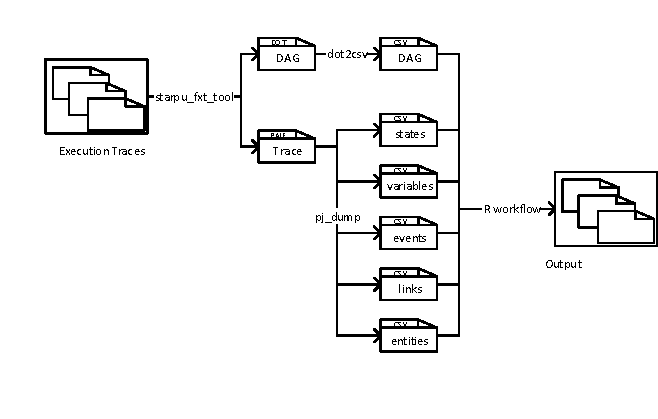
\includegraphics[width=1\textwidth]{./img/step1-final.pdf}}
 \caption{\emph{Workflow} de pré-processamento do StarVZ.}
 \label{fig:starvz-workflow1}
\end{figure}

Inicialmente, as saídas do StarPU, que são arquivos em um formato binário, são 
transformadas e exportadas através da ferramenta \textbf{starpu\_fxt\_tool} para dois 
arquivos: DAG no formato DOT e Trace no formato PAJE. Essa etapa gera
eventos com informação de data e hora, que descrevem o comportamento da aplicação para todos os recursos 
envolvidos. Além disso, também são gerados dados sobre o \emph{runtime} do StarPU, como 
número de tarefas submetidas, número de tarefas prontas, arquitetura da plataforma, etc.

A segunda etapa consiste em uma verificação de integridade estrutural e temporal dos
arquivos trace. Ela é executada via \textbf{pj\_dump}, gerando cinco arquivos: o arquivo states 
possui informações sobre as tarefas executadas e seu comportamento no \emph{runtime}; variables
consiste em métricas de performance da plataforma e runtime; events possui informações sobre a 
utilização de recursos; links contém dados sobre comunicação MPI; e as informações de plataforma 
são registradas no arquivo entities. O DAG também passa por uma conversão e por fim, todos os 
arquivos são gravados no formato \emph{Comma-Separated Value} (CSV).

Finalmente, os dados escritos em CSV são lidos, filtrados, agregados e combinados em 
uma ferramenta implementada sobre R, utilizando-se bibliotecas oriundas do pacote 
\textbf{tidyverse} para a manipulação de dados. As saídas são escritas no formato \emph{FEATHER}
\cite{ref:feather}.

A segunda fase do \emph{workflow} inicia pela leitura das saídas da fase anterior. Cada arquivo
torna-se um \emph{data frame}, e os dados da execução inteira são unificados em uma estrutura.
É possível ter múltiplos \emph{traces} de aplicações sendo analisados em paralelo
para comparação, basta executar essa fase novamente com entradas diferentes e 
elas posteriormente serão combinadas em uma única visualização. A criação dos gráficos ainda 
possui processamento de dados, o que traz alguma flexibilidade para as visualizações. Na 
etapa final dessa fase, o usuário parametriza o sistema com um arquivo configuração, no formato
YAML, para que a montagem da visualização seja customizada. Finalmente, o usuário pode analisar os 
gráficos gerados pela ferramenta.

Tratando-se de otimizações, a segunda fase do \emph{workflow} leva em torno de 2 minutos para ler os
arquivos FEATHER e gerar uma visualização. Portanto, a primeira fase do \emph{workflow} é a que mais carece de otimizações.
No experimento citado em \citet{ref:starvz}, a execução da starpu\_fxt\_tool levou em torno de 10 minutos, a 
pj\_dump levou em torno de 9 minutos e as ferramentas R que fazem as junções, limpeza e filtragem levou 13 minutos.



\section{Trabalhos Relacionados}\label{sect:related-work}